\documentclass[
  bibliography=totoc,     % Literatur im Inhaltsverzeichnis
  captions=tableheading,  % Tabellenüberschriften
  titlepage=firstiscover, % Titelseite ist Deckblatt
]{scrartcl}

% Paket float verbessern
\usepackage{scrhack}

% Warnung, falls nochmal kompiliert werden muss
\usepackage[aux]{rerunfilecheck}

% unverzichtbare Mathe-Befehle
\usepackage{amsmath}
% viele Mathe-Symbole
\usepackage{amssymb}
% Erweiterungen für amsmath
\usepackage{mathtools}

% Fonteinstellungen
\usepackage{fontspec}
% Latin Modern Fonts werden automatisch geladen
% Alternativ zum Beispiel:
%\setromanfont{Libertinus Serif}
%\setsansfont{Libertinus Sans}
%\setmonofont{Libertinus Mono}

% Wenn man andere Schriftarten gesetzt hat,
% sollte man das Seiten-Layout neu berechnen lassen
\recalctypearea{}

% deutsche Spracheinstellungen
\usepackage[ngerman]{babel}


\usepackage[
  math-style=ISO,    % ┐
  bold-style=ISO,    % │
  sans-style=italic, % │ ISO-Standard folgen
  nabla=upright,     % │
  partial=upright,   % ┘
  warnings-off={           % ┐
    mathtools-colon,       % │ unnötige Warnungen ausschalten
    mathtools-overbracket, % │
  },                       % ┘
]{unicode-math}

% traditionelle Fonts für Mathematik
\setmathfont{Latin Modern Math}
% Alternativ zum Beispiel:
%\setmathfont{Libertinus Math}

\setmathfont{XITS Math}[range={scr, bfscr}]
\setmathfont{XITS Math}[range={cal, bfcal}, StylisticSet=1]

% Zahlen und Einheiten
\usepackage[
  locale=DE,                   % deutsche Einstellungen
  separate-uncertainty=true,   % immer Unsicherheit mit \pm
  per-mode=symbol-or-fraction, % / in inline math, fraction in display math
]{siunitx}

% chemische Formeln
\usepackage[
  version=4,
  math-greek=default, % ┐ mit unicode-math zusammenarbeiten
  text-greek=default, % ┘
]{mhchem}

% richtige Anführungszeichen
\usepackage[autostyle]{csquotes}

% schöne Brüche im Text
\usepackage{xfrac}

% Standardplatzierung für Floats einstellen
\usepackage{float}
\floatplacement{figure}{htbp}
\floatplacement{table}{htbp}

% Floats innerhalb einer Section halten
\usepackage[
  section, % Floats innerhalb der Section halten
  below,   % unterhalb der Section aber auf der selben Seite ist ok
]{placeins}

% Seite drehen für breite Tabellen: landscape Umgebung
\usepackage{pdflscape}

% Captions schöner machen.
\usepackage[
  labelfont=bf,        % Tabelle x: Abbildung y: ist jetzt fett
  font=small,          % Schrift etwas kleiner als Dokument
  width=0.9\textwidth, % maximale Breite einer Caption schmaler
]{caption}
% subfigure, subtable, subref
\usepackage{subcaption}

% Grafiken können eingebunden werden
\usepackage{graphicx}

% schöne Tabellen
\usepackage{booktabs}

% Verbesserungen am Schriftbild
\usepackage{microtype}

% Literaturverzeichnis
\usepackage[
  backend=biber,
]{biblatex}
% Quellendatenbank
\addbibresource{lit.bib}
%\addbibresource{programme.bib}

% Hyperlinks im Dokument
\usepackage[
  german,
  unicode,        % Unicode in PDF-Attributen erlauben
  pdfusetitle,    % Titel, Autoren und Datum als PDF-Attribute
  pdfcreator={},  % ┐ PDF-Attribute säubern
  pdfproducer={}, % ┘
]{hyperref}
% erweiterte Bookmarks im PDF
\usepackage{bookmark}

% Trennung von Wörtern mit Strichen
\usepackage[shortcuts]{extdash}

\author{
  Thomas-Christopher Ogasa \\
  \href{mailto:thomas.ogasa@tu-dortmund.de}{thomas.ogasa@tu-dortmund.de}
  \\
  \\
  Jiayue Ruan \\
  \href{mailto:jiayue.ruan@tu-dortmund.de}{jiayue.ruan@tu-dortmund.de}
}
\publishers{TU Dortmund – Fakultät Physik}

\renewcommand{\d}{\symup{d}}
\newcommand{\diff}[2]{\frac{\symup{d} #1}{\symup{d} #2}}
\newcommand{\e}{\symup{e}}
\newcommand{\idx}[1]{_{\symup{ #1 }}}
\newcommand{\pdiff}[2]{\frac{\partial #1}{\partial #2}}
\newcommand{\s}{ß}


\subject{V44}
\title{Röntgenreflektrometrie}
\date{
  Durchführung: 19.06.2023
  \hspace{3em}
  Abgabe: 23.07.2023
}
\usepackage[aux]{rerunfilecheck}

\usepackage{fontspec}
\usepackage{siunitx}

\usepackage[ngerman]{babel}

\usepackage[unicode]{hyperref}
\usepackage{bookmark}
\usepackage{booktabs}
\usepackage{import}
\usepackage{amsmath}

\usepackage{scrhack}

\usepackage[aux]{rerunfilecheck}

\usepackage{fontspec}

\usepackage[ngerman]{babel}

\usepackage{amsmath}
\usepackage{amssymb}
\usepackage{mathtools}

\usepackage{booktabs}

\usepackage[unicode]{hyperref}
\usepackage{bookmark}
\usepackage{svg}

\begin{document}

\maketitle
\thispagestyle{empty}
\tableofcontents
\newpage


\section{Zielsetzung}
In diesem Versuch soll die Dichte, Rauigkeit und Schichtdicke eines Polysterolschicht
mithilfe der Röntgenreflektrometrie bestimmt werden.

\section{Theorie}

\subsection{Erzeugung von Röntgenstrahlung}
Elektromagnetische Wellen, die in einem Wellenlängenbereich von ungefähr $10^{-9}\,\unit{\meter}$ bis $10^{-11}\,\unit{\meter}$
liegen, werden als Röntgenstrahlen bezeichnet. Sie haben entsprechend eine Energie von ca. $100\,\unit{\electronvolt}$ bis $250\,\unit{\kilo\electronvolt}$.
Die Röntgenstrahlung im Versuch wird in einer Röntgenröhre erzeugt.

\begin{figure}[H]
  \centering
  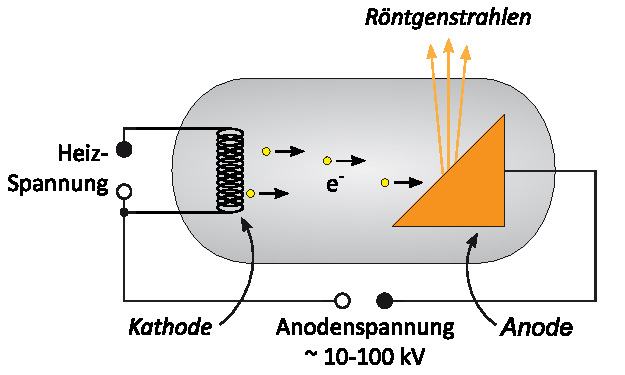
\includegraphics[scale=0.75]{röntgenröhre.pdf}
  \caption{Erzeugung von Röntgenstrahlung in einer Röntgenröhre \cite{uni_goettingen}.}
  \label{fig:roentgenroehre}
\end{figure}
\noindent
Zuerst wird durch das Erhitzen der Glühkathode ($10\,\unit{\kilo\volt}-100\,\unit{\kilo\volt}$) Elektronen freigesetzt (glühelektrischer Effekt).
Die Erzeugung von Röntgenstrahlung in einer Röntgenröhre basiert prinzipiell auf der Beschleunigung von Elektronen 
von der Glühkathode zur Anode. Wenn die Elektronen auf die Anode treffen, entstehen Bremsstrahlung 
und charakteristische Röntgenstrahlung. Die Bremsstrahlung resultiert aus der Abbremsung der Elektronen 
durch das Coulombfeld der Atomkerne, während die charakteristische Röntgenstrahlung durch den Übergang der Elektronen in den 
Atomhüllen erzeugt wird. In Abbildung \ref{fig:roentgenroehre} ist der schematische Aufbau einer 
Röntgenröhre zu sehen.




\subsection{Röntgenstrahlung an einer Grenzfläche}
In Abbildung \ref{fig:reflection_transmission} wird ein Strahl an einer Grenzfläche reflektiert und transmittiert. Dabei 
wird der Einfalls-, bzw. Ausfallswinkels als $\phi$ bezeichnet und $\varphi$ ist der Winkel zwischen der transmittierten Welle und der Grenzebene.
Im Folgenden wird $\phi$ durch $\alpha$ ersetzt und $\varphi$ durch $\alpha\idx{t}$. Eine Unterscheidung zwischen dem Ein- und Ausfallswinkel ist 
nicht zwingend nötig, da diese nach dem Reflektionsgesetz identisch sind.
\begin{figure}[H]
  \centering
  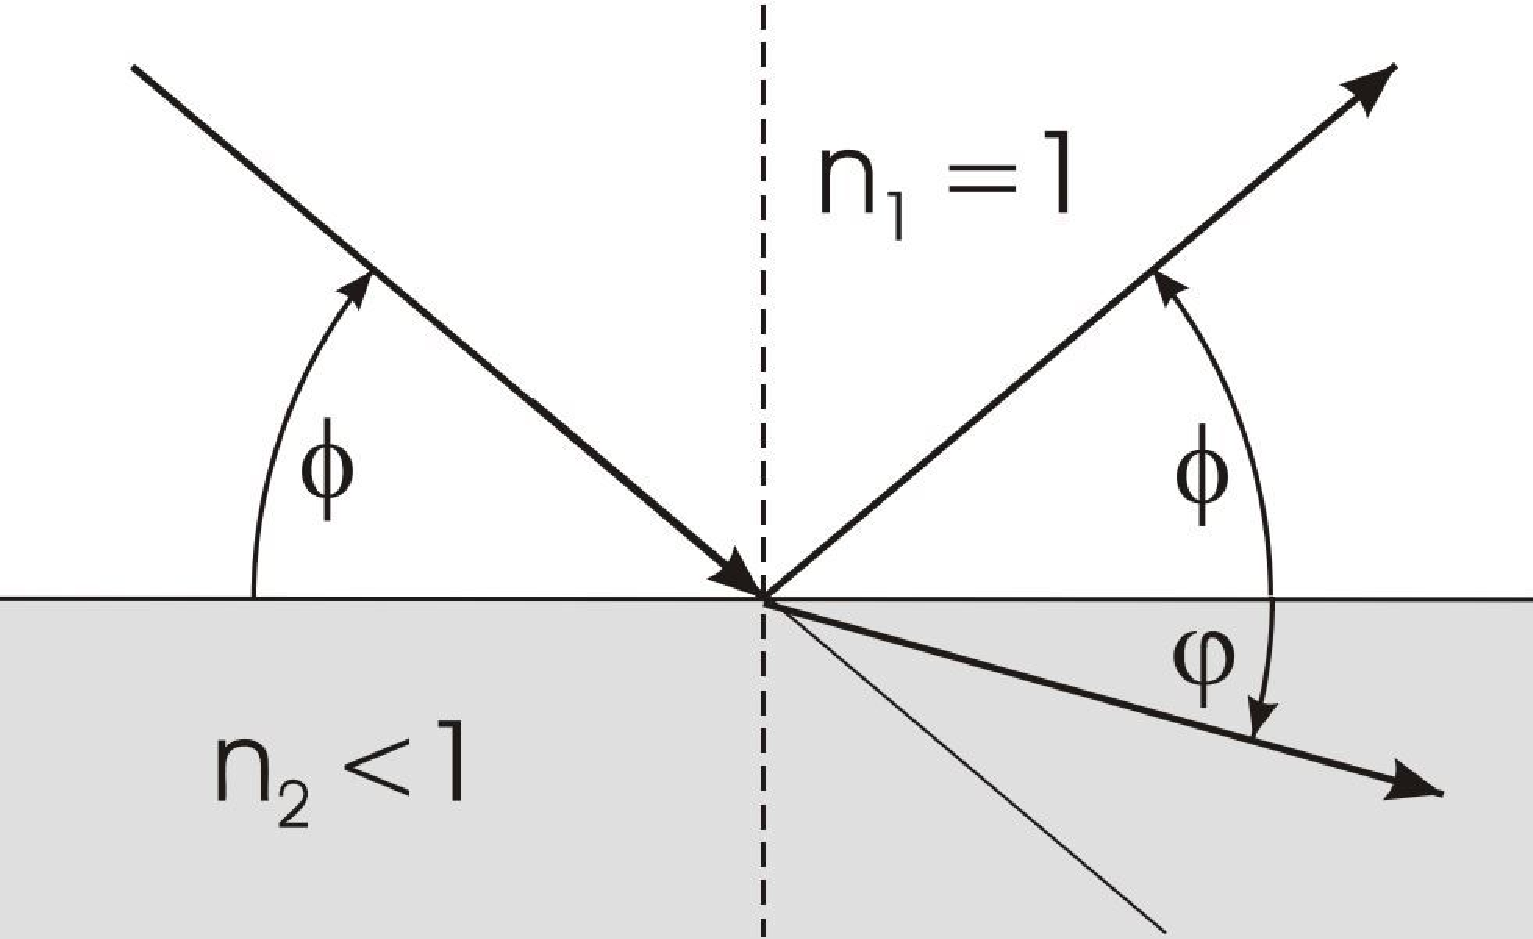
\includegraphics[scale=0.25]{rt.pdf}
  \caption{Lichtstrahl wird an einer Oberfläche reflektiert und transmittiert \cite{uni_giessen}.}
  \label{fig:reflection_transmission}
\end{figure} 
\noindent
Der Brechungsindex beschreibt die Stärke der Brechung von Licht
beim Übergang von einem Medium in ein anderes. Die Lichtgeschwindigkeit im Vakuum
ist eine feste Größe, jedoch ist die Geschwindigkeit in Materie materialspezifisch. Der
Brechungsindex gibt das Verhältnis zwischen der Lichtgeschwindigkeit in Materie und
der Lichtgeschwindigkeit im Vakuum an.
In Falle von Röntgenstrahlung ist der Brechungsindex
\begin{equation}
  n= 1 - \delta + i \beta , 
\end{equation}
wobei $\beta$ und $\delta$ die materialspezifische Absorptionkonstante und Dispersion (Größenordnung $10^{-6}$) sind.
Ab einem kritischen Winkel $\alpha\idx{C}$ tritt Totalreflexion auf. Diese ist 
\begin{equation}
  \alpha\idx{C} \approx \sqrt{2 \delta} = \lambda \sqrt{\frac{\rho r\idx{e}}{\pi}}
  \label{eq:kritisch}
\end{equation}
unter der Annahme von kleinen Winkeln. Hier ist $\lambda$ die Wellenlänge, $\rho$ die Elektronendichte des Stoffes und 
$r\idx{e}$ der Elektronenradius.
Um das Amplitudenverhältnis des reflektierten und transmittierten Anteil des Lichts, wenn es auf eine Grenzfläche zwischen zwei 
verschiedene optische Medien trifft, zu beschreiben, 
werden Fresnelgleichungen herangezogen. Dabei wird zwischen senkrecht (s) und parallel (p) polarisiertes Licht unterschieden.
Bei Röntgenstrahlung können die Polarisationseigenschaften jedoch vernachlässigt werden, da sie unpolarisiert sind und keine bevorzugte 
Ausrichtung besitzen. So kann bei Betrachtung von Röntgenstrahlung angenommen werden, dass beide Polarisationsanteile ungefähr gleich sind.
Für den Reflektions-, bzw. Transmissionskoeffizient gilt
\begin{equation}
  r= \frac{n\idx{1} \sin \alpha\idx{i} - n\idx{2} \sin \alpha\idx{t}}{n\idx{1} \sin \alpha\idx{i} + n\idx{2} \sin \alpha\idx{t}}
\end{equation}
und
\begin{equation}
  t= \frac{2n\idx{1} \sin \alpha\idx{i}}{{n\idx{1} \sin \alpha\idx{i} + n\idx{2} \sin \alpha\idx{t}}}.
\end{equation}
Hierbei stehen $n\idx{1}$ und $n\idx{2}$ für die Brechungsindizes des ersten, bzw. zweiten Mediums.
Die Intensität des Lichtstrahls ist proportional zum Quadrat der Feldstärke. Die Reflektivität ist das Verhältnis 
zwischen der reflektierten Strahlintensität $I\idx{r}$ und der einfallenden Strahlintensität $I\idx{e}$ und wird durch 
\begin{equation*}
  R = \frac{I\idx{r}}{I\idx{e}} =|r|^2 
\end{equation*}
ausgedrückt.




\subsection{Reale Proben}
Bisher wurde in der Reflexionsbetrachtung von ideal glatten Grenzflächen und einschichtigen Proben ausgegangen. Allerdings trifft diese Annahme 
nicht auf reale Grenzflächen zu. Die Eigenschaften realer Proben werden in folgende Abschnitte behandelt.

\subsubsection{Mehrschichtsysteme}
In diesem Abschnitt werden Mehrschichtsysteme behandelt. In Abbildung \ref{fig:reflectivity} ist
Reflektivit eines Siliziumwafers mit einem Polysterolschicht bei einer Wellenlänge von $\lambda = 1,54\,\unit{\angstrom}$ dargestellt. 
In dem Subplot wird ein Bereich vergrößert und die kritischen Winkel $\alpha\idx{C}$ jeweils für den Siliziumwafer und die Polysterolschicht gekennzeichnet.
Für ein Einfallswinkel $\alpha\idx{i} > \alpha\idx{C}$ findet keine Totalreflexion mehr statt, so dass die Reflektivität danach drastisch abnimmt.
\begin{figure}[H]
  \centering
  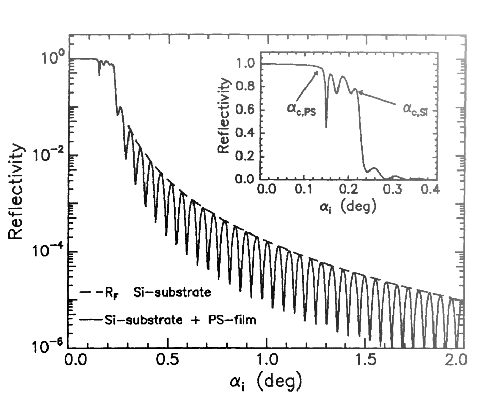
\includegraphics[scale=1.2]{reflectivity_plot.pdf}
  \caption{Reflektivit eines Siliziumwafers mit einem Polysterolschicht anhängig vom Einfallswinkel der Strahlung \cite{tolan}.}
  \label{fig:reflectivity}
\end{figure}
\noindent
Zudem sind Oszillationen zu erkennen, die aufgrund von Interferenzeffekte an den Grenzflächen der beiden Schichten auftreten.
Diese werden auch als Kiessig-Oszillationen bezeichnet. Sie entstehen, indem ein Teil der Strahlung, der das erste Medium durchdringt, 
an der Grenzfläche zum zweiten Medium reflektiert wird. Dieser reflektierte Anteil interferiert dann mit dem Teil der Strahlung, der 
bereits am ersten Medium reflektiert wurde. Über die Gleichung 
\begin{equation}
d = \frac{\lambda}{2\upDelta \alpha\idx{i}}
\label{eq:schicht}
\end{equation}
kann die Schichtdicke berechnet werden. Dabei ist $\upDelta \alpha\idx{i}$ der Abstand zwischen zwei Minima/Maxima.
Bestehen Systeme aus mehr als zwei Schichten, überlagern sich die Oszillationen. Um diese Überlagerung zu quantifizieren, wird der 
Parratt-Algorithmus verwendet. Dieser ist ein rekursives Verfahren zur Beschreibung eines Mehrschichtsystems. 
In Abbildung \ref{fig:multischichtsystem} ist ein solches mit $N$-Schichten abgebildet. Die Welle wird an jeder Grenzfläche zum Teil 
reflektiert (blau) und transmittiert (rot). $T\idx{j}$ und $R\idx{j}$ sind dabei die Amplituden für den transmittierten, bzw. reflektierten 
Strahl.
\begin{figure}[H]
  \centering
  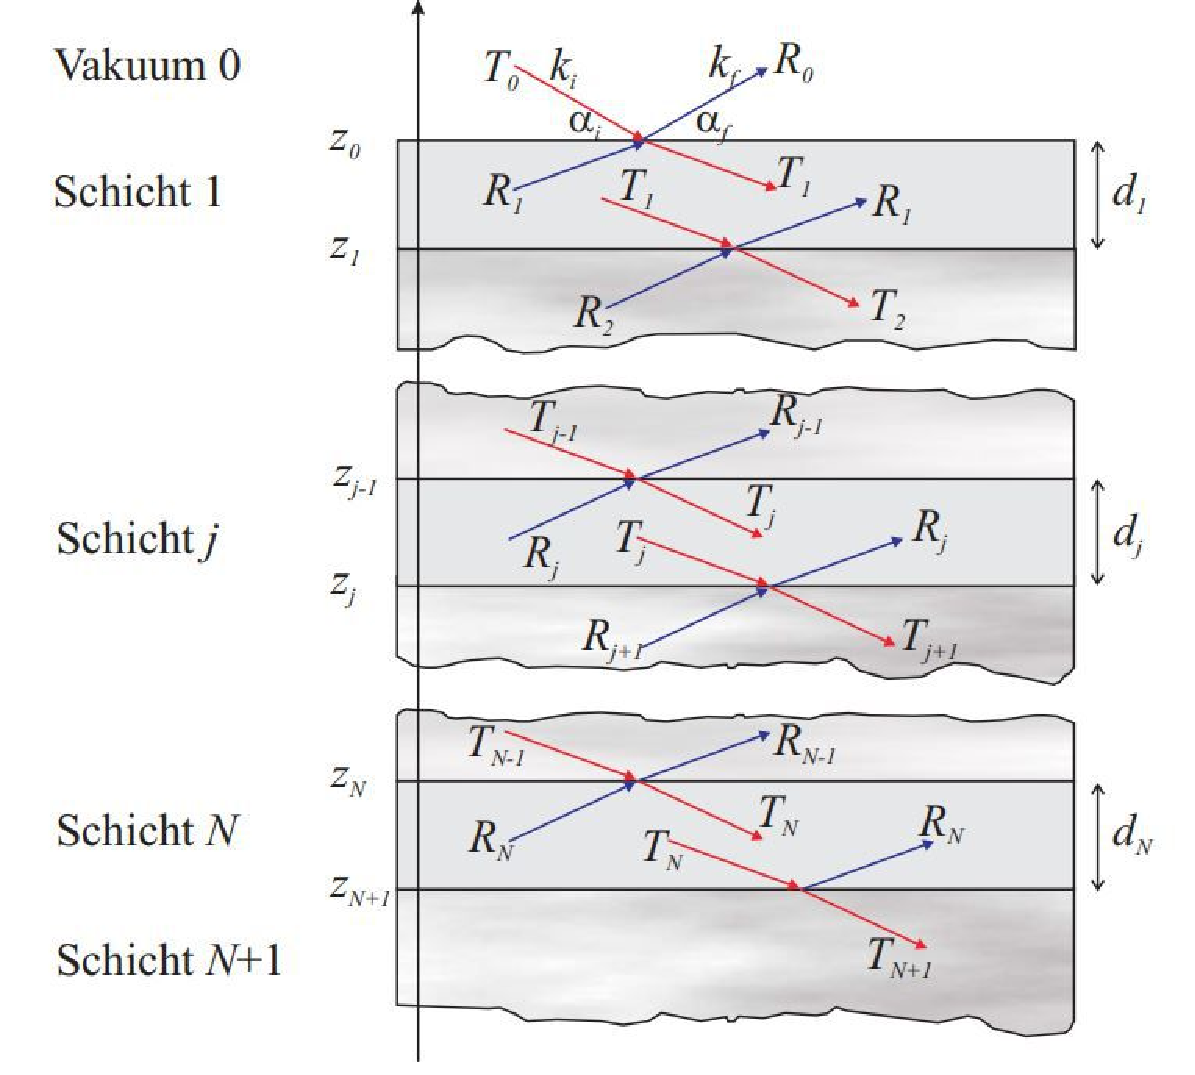
\includegraphics[scale=0.4]{mehrschichtsystem.pdf}
  \caption{Reflexion und Brechung an einem Mehrschichtsystem mit $N$ Grenzschichten \cite{Bachelorarbeit_Bertram}.}
  \label{fig:multischichtsystem}
\end{figure}
\noindent
Der Parratt-Algorithmus durchläuft rekursiv alle Schichten, beginnend mit der untersten Schicht (Schicht $N$). 
Es wird angenommen, dass die Dicke der darunter liegenden Schicht deutlich größer als die Tiefe ist, auf die Röntgenstrahlen 
in ein Material eindringen können. Daraus folgt die Bedingung $R\idx{N,N+1}=0$. Die Welle wird nämlich an der letzten 
Grenzfläche transmittiert (und reflektiert), jedoch nicht wieder von einer weiteren Schicht zurückreflektiert. 
Ausgehend von der untersten Schicht kann jeweils das Verhältnis zwischen $T\idx{j}$ und $R\idx{j}$ 
mit 
\begin{equation}
  X\idx{j} = \frac{R\idx{j}}{T\idx{j}} = \frac{r\idx{j,j+1} + X\idx{j+1} \exp({2ik\idx{j+1,z}d\idx{j}})}{1+ r\idx{j,j+1} X\idx{j+1} \exp({2ik\idx{j+1,z}d\idx{j}})} \exp({-2ik\idx{j,z}d\idx{j}})
\end{equation}
ermittelt werden. Hierbei ist $d\idx{j}$ die Dicke der $j$-ten Schicht und 
\begin{equation}
  r\idx{j,j+1} = \frac{k\idx{k,z} - k\idx{j+1,z}}{k\idx{k,z} + k\idx{j+1,z}}
\end{equation}
der Fresnel-Koeffizient für die Schichten $j$ und $j+1$ und 
\begin{equation}
  k\idx{z,j} = k \sqrt{n^2\idx{j}-\cos^2\alpha\idx{i}}
\end{equation}
die $z$-Komponente des $j$-ten Wellenvektors.


\subsubsection{Rauigkeit}
Reale Proben haben keine ideal glatte Grenzflächen, was jedoch bis jetzt in der Theorie angenommen wurde. 
Um dies zu korrigieren, werden die Fresnel-Koeffizienten modifiziert
\begin{equation}
  \tilde{r}\idx{j+1,j} = r\idx{j,j+1} \exp(-2k\idx{z,j}k\idx{z,j+1} \sigma^2\idx{j})
\end{equation}
und
\begin{equation}
  \tilde{t}\idx{j+1,j} = t\idx{j,j+1} \exp \left ((k\idx{z,j}-k\idx{z,j+1})^2 \frac{\sigma^2\idx{j}}{2} \right ),
\end{equation}
wobei $\sigma$ für die Rauigkeit steht. Wird $\sigma=0$ eingesetzt, so resultierten wieder die vorherigen Fresnel-Koeffizienten
für ideal glatte Ebenen. Des Weiteren wird angenommen, dass $\sigma << d$ ist.
Das Auswerten mit dem Parratt-Algorithmus erfolgt mit diesen angepassten Fresnel-Koeffizienten.







\subsection{Korrektur Geometriefaktor}
Der Röntgenstrahl trifft auf die Probenoberfläche und erst ab einem bestimmten Geometriewinkel
\begin{equation*}
  \alpha\idx{G} = \mathrm{arcsin} \left ( \frac{d\idx{0}}{D} \right )
\end{equation*}
findet die vollständige Reflexion des Strahls statt. Bei sehr geringen Winkeln wird der Strahl nicht vollständige reflektiert.
Zusätzliche Bedingungen hinsichtlich des Einfallswinkels sind erforderlich, um weitere Berechnungen durchzuführen.
Der sogenannte Geometriefaktor wird eingeführt und ist als
\begin{equation*}
  G = 
\begin{cases}
1 & \alpha\idx{i} \geq \alpha\idx{G} \\
\frac{D \sin \alpha\idx{i}}{d\idx{0}} & \, \alpha\idx{i} < \alpha\idx{G}, \\
\end{cases}
\end{equation*}
gegeben. Dabei entspricht $D$ die Länge der Probe, $d\idx{0}$ die gesamte Strahlbreite und $D \sin \alpha\idx{i}$ damit die 
effektive Strahlbreite.
\section{Aufbau und Durchführung}



\section{Auswertung}
\subsection{Detektor-scan}
Der Detektor-scan scan wird wie in der Durchführung beschrieben durchgeführt. An die Mess wurde eine Funktion der Form 
\begin{equation}
    I(\alpha)= I\idx{max}\cdot \e^{-(\frac{x-\mu}{\sigma})^2}
\end{equation}
angenähert. Die kurve is zu sehen in \ref{fig:decscan}. Die dabei resultierenden parameter sowie die Halbwertsbreite FWHM ist
\input{build/paramsdecScan.tex}
wobei die Halbwertsbreite mit 
\begin{equation}
    FWHM = \sqrt{8 \text{ln}(2)}(\sigma)
\end{equation}
bestimmt wurde.
\begin{figure}
    \centering
    \includegraphics[width = 11.2cm]{build/plotdecScan.pdf}
    \caption{Messdaten des Detektor-scans, daran eine Gausskurve angenähert.}
    \label{fig:decscan}
\end{figure}
\subsection{Z-scan}
\label{chap:zscan}
Die Messwerte des Z-scans sind in Abbildung \ref{fig:zscan} zu sehen. Die Strahlenbreite, welche abzulesen war, beträgt
\input{build/ergzScan.tex}
\begin{figure}
    \centering
    \includegraphics[width = 11.2cm]{build/plotzScan.pdf}
    \caption{Messdaten des Z-scans. Identifiezierte Strahlenbreite ist des weiteren eingetragen.}
    \label{fig:zscan}
\end{figure}
\subsection{Rocking-scan}
Zur bestimmung des Geometriefaktor wurde der Rocking-scan durchgeführt. In Abbildung \ref{fig:rocking} sind die Messwerte zu sehen.
\begin{figure}
    \centering
    \includegraphics[width = 11.2cm]{build/plotrockingScan.pdf}
    \caption{Messdaten des Rocking-scan sowie die daraus Identifiezierten Geometriewinkel.}
    \label{fig:rocking}
\end{figure}
Die enden des zu Geometriefaktor korrigierenden bereichs wurden aus Abbildung \ref{fig:rocking} abgelesen. Der Geometriewinkel wurde als
arithmetisches Mittel beider Winkel bestimmt. Der daraus resultierte Wert ist
\input{build/parrockingScan.tex}
Mit der Strahlenbreite aus Kapitel \ref{chap:zscan}, wurde der theoretische Geometriewinkel 
\begin{equation}
    \alpha\idx{theorie} = \text{arcsin}\left(\frac{d\idx{0}}{D}\right) = 1.777°,
\end{equation}
mit $D=20\,\si{\milli\meter}$. Auf grund der eindeutigen Abweichung, des theoretischen Wertes und dem experimentel bestimmten, wird im folgenden
der $\alpha\idx{theorie}$ für die Geometriefaktorkorrektur verwendet.
\subsection{Reflektivitäts-scan}
Bei der Reflektivitätsmessung wird die Schichtdicke $d\idx{0}$ sowie der kritische Winkel $\alpha\idx{c}$ bestimmt. Dazu werden die Messwerte
zunächst korrigiert mit den Messwerten eines analogen difusen Scans. Diese Messwerte sind in Abbildun \ref{fig:refl} zu sehen. 
\begin{figure}
    \centering
    \includegraphics[width = 11.2cm]{build/plotreflecScan.pdf}
    \caption{Messdaten des Reflektions-scan, mit und ohne Geometriefaktorkorrektur. Des weiteren ist der kritische Winkel eingetragen.}
    \label{fig:refl}
\end{figure}
Des weiteren sind die Messdaten, welche mit dem Geometriefaktor korrigiert wurden, in gleicher Abbildung zu sehen. Aus den gemessenen 
Intensitäten wurde die Reflektivität errechnet mittels
\begin{equation}
    R = \frac{5I}{I\idx{max}}
\end{equation}
bestimmt. Die minima wurden visuell bestimmt, und das arithmetische Mittel der differenzen wurde berechnet. Aus diesem Mittelwert wird die 
Schichtdicke mittels Formel \eqref{eq:schicht} bestimmt. Die daraus resultierten ergebnisse sind 
\input{build/ergreflecScan.tex}
Zur Bestimmung der Schichtdicke des Polysterols wurde die Wellenlänge der $K\idx{\alpha, 1} = 1.541\,\si{\angstrom}$ verwendet.
\subsection{Bestimmung des Dispersionsprofil mittels des Parratt-Algorithmus}
Auf den gleichen Daten wie im vorherigen Kapitel wird der Parratt-Algorithmus angewendet. Das wird durchgeführt, um die das Dispersionsprofil
der Probe zu bestimmen. Der Parratt-Algorithmus is für raue Oberflächen angepasst, und kann entsprechend auch ein Maß, wie rau die Oberfläche
ist, abschätzen. Es wurden zwei Schichten betrachten, eine Polysterolschicht auf einer Siliziumschicht. Die Luft ist als Vakuum angenähert.
\begin{figure}
    \centering
    \includegraphics[width = 11.2cm]{build/plotparratt.pdf}
    \caption{Messdaten des Reflektions-scan korrigiert Geometriefaktorkorrektur. Eine Parrattkurve wurde händisch an die Messwerte angenähert.}
    \label{fig:refl}
\end{figure}
Es wurden die Parameter der Parrattkurve händisch an die Messdaten angenähert. Die dabei gefunden Werte sind
\begin{equation}
    \begin{aligned}
        \delta\idx{2} &= 7.6\cdot 10^{6} \\
        \delta\idx{3} &= 8.077\cdot 10^{6} \\
        \sigma\idx{1} &= 2.688\cdot 10^{9} \\
        \sigma\idx{2} &= 4.829\cdot 10^{10} \\
        b\idx{1} &= 3.863\cdot 10^{7} \\
        b\idx{2} &= 1.483\cdot 10^{5} \\
        d\idx{2} &=  813.9\,\si{\angstrom}.
    \end{aligned}
\end{equation}
Aus den Parametern kann anschließend der kritische Winkel mit Formel \eqref{eq:kritisch} bestimmt. Die kritischen Winkel betragen
\begin{equation}
    \begin{aligned}
        \alpha\idx{c, exp, Polysterol} &= 0.0039\,° \\
        \alpha\idx{c, exp, Silizium} &= 0.0040\,°
    \end{aligned}
\end{equation}
\section{Diskussion}
Beim detektor-scan wurde die Parameter 
\input{build/paramsdecScan.tex}
ermittelt. Wiederrum beim Z-scan wurde eine Strahlenbreite von 
\input{build/ergzScan.tex} 
bestimmt. Da es für diese Werte keine Theoriewerte, zum vergleich gibt kann keine Aussage über die Güte der Messung getroffen werden.
Bei dem Rocking-scan wurde ein Geometriewinkel von $\alpha{G} = 2.26\,°$ ermittelt. Verglichen mit dem Theoriewert $\alpha\idx{G, Theorie} = 1.777$
hat dieser Wert eine abweichung von ca $27.2\,\%$. Da diese Werte keine Unsicherheiten haben, ist eine eindeutige Aussage nicht möglich,
die hoche relative Abweichung deutet allerdings auf eine Fehlerhafte Justage.\\
Die messdaten der Reflektionmessung betohnt die bisherige Vermutung, da das erwartete Plateau, klein und undeutig ist. Vergleicht man 
die Ergebnisse der Schichtdicke, vom Reflektionscan und der Parrattkurve, 
\begin{equation}
\begin{aligned}
    d\idx{0} &= (959.70 \pm 0.71)\,\si{\angstrom} \\
    d\idx{0} &= 813.9\,\si{\angstrom} \\
\end{aligned}
\end{equation}
ist offensichtilich, dass diese nicht mit einander Übereinstimmen. Die Abweichung beträgt $(17.91 \pm0.09)\,\%$. Dies ließe sich mit dem 
hohen Raschen in den Oszillationen erklären. Dadurch, dass die Unsicherheit nur aus der Abweichung der Differenzen bestimmt wurde,
ist diese eindeutig eine Unterschätzung des realen Fehlers.
Die Parameter der Parrattkurve welche mit Literaturwerten \cite{V44} vergleichbar sind, sind die $\delta$ werte. Diese sowie die 
korrespondierenden Literaturwerte sind:
\begin{equation}
    \begin{aligned}
        \delta\idx{2, Parratt} &= 7.6\cdot 10^{6} \\
        \delta\idx{3, Parratt} &= 8.077\cdot 10^{6} \\
        \delta\idx{2, Theorie} &= 5\cdot 10^{6} \\
        \delta\idx{3, Theorie} &= 7.6\cdot 10^{6}. \\
    \end{aligned}
\end{equation}
Die Abweichungen hier sind $r\idx{2} = 52\,\%$ und $r\idx{3} = 6\,\%$. Hier ist aufzufallen, dass der Wert für $\delta\idx{3}$ eine geringe
und $\delta\idx{2}$ eine vergleichsweise hohe Abweichung hat. Aufgrund der händischen Annäherung an die Messwerte, fehlen jedoch die 
Ungenauigkeiten, was einen echten Vergleich unmöglich macht. Dennoch die große Abweichung von $\delta\idx{2}$ spricht erneut für eine 
Fehlerhafte Justage. Die Ergebnisse des Parrattalgorithmus, welche nicht mit Literaturwerten vergleichbar sind, sind 
\begin{equation}
    \begin{aligned}
        \sigma\idx{1} &= 2.688\cdot 10^{9} \\
        \sigma\idx{2} &= 4.829\cdot 10^{10} \\
        b\idx{1} &= 3.863\cdot 10^{7} \\
        b\idx{2} &= 1.483\cdot 10^{5} \\
        d\idx{2} &=  813.9\,\si{\angstrom}.
    \end{aligned}
\end{equation}




\nocite{*}
\printbibliography


\end{document}
